\documentclass[letterpaper,11pt]{article}
\oddsidemargin -1.0cm \textwidth 17.5cm

\usepackage[utf8]{inputenc}
\usepackage[activeacute,spanish, es-lcroman]{babel}
\decimalpoint
\usepackage{amsfonts,setspace}
\usepackage{amsmath}
\usepackage{amssymb, amsmath, amsthm}
\usepackage{comment}
\usepackage{float}
\usepackage{amssymb}
\usepackage{dsfont}
\usepackage{anysize}
\usepackage{multicol}
\usepackage{enumerate}
\usepackage{graphicx}
\usepackage[left=1.5cm,top=2cm,right=1.5cm, bottom=1.7cm]{geometry}
\setlength\headheight{1.5em} 
\usepackage{fancyhdr}
\usepackage{multicol}
\usepackage{hyperref}
\usepackage{wrapfig}
\usepackage{subcaption}
\usepackage{siunitx}
\usepackage{cancel}
\usepackage{mdwlist}
\usepackage{svg}
\usepackage{tcolorbox}
\pagestyle{fancy}
\fancyhf{}
\renewcommand{\labelenumi}{\normalsize\bfseries P\arabic{enumi}.}
\renewcommand{\labelenumii}{\normalsize\bfseries (\alph{enumii})}
\renewcommand{\labelenumiii}{\normalsize\bfseries \roman{enumiii})}


\begin{document}

\fancyhead[L]{\itshape{Facultad de Ciencias F\'isicas y Matem\'aticas}}
\fancyhead[R]{\itshape{Universidad de Chile}}

\begin{minipage}{11.5cm}
    \begin{flushleft}
        \hspace*{-0.6cm}\textbf{FI1000-1 Introducción a la Física Clásica}\\
        \hspace*{-0.6cm}\textbf{Profesora:} Jocelyn Dunstan\\
        \hspace*{-0.6cm}\textbf{Auxiliar:} Alejandro Silva\\
        \hspace*{-0.6cm}\textbf{Ayudantes:} Macarena Muñoz \& Catalina Vargas\\
    \end{flushleft}
\end{minipage}

\begin{picture}(2,3)
    \svgpath{../}  % descomentar si se agrega a carpeta "auxiliares"/"ejercicios"
    \put(366, 10){\includesvg[scale=0.31]{img/dfi.svg}}
\end{picture}

\begin{center}
	\LARGE\textbf{Auxiliar \#11}\\
	\Large{Repaso C2}
\end{center}

\vspace{-1cm}
\begin{enumerate}\setlength{\itemsep}{0.4cm}

\rfoot[]{pág. \thepage}

\item[]

\item Una partícula colisiona a una segunda partícula de igual masa que estaba inicialmente en reposo. Si colisionan elásticamente sobre un plano horizontal libre de roce, determine el ángulo $\phi$ de salida de la partícula inicialmente en reposo si la primera partícula se desvía un ángulo $\theta$ con respecto a la dirección que traía antes de la colisión.

\begin{figure}[htbp]
  \centering
  \svgpath{../../2021-1/Imagenes/aux11}
  \includesvg[width=0.4\linewidth]{pelotas.svg}
\end{figure}

\item Se lanza un proyectil con una rapidez inicial $v_0$, formando un ángulo de $\theta_0$ con respecto a la horizontal. En el punto más alto de su vuelo, el proyectil explota rompiéndose en dos partes, una de las cuales tiene el doble de masa que la otra. Los dos fragmentos salen inicialmente despedidos en la dirección horizontal (como se indica en la figura), y aterrizan simultáneamente. Si el fragmento más ligero aterriza a una distancia $L$ del punto de lanzamiento, determine la posición $\ell$ donde aterrizará el otro fragmento.

\begin{figure}[H]
    \centering
    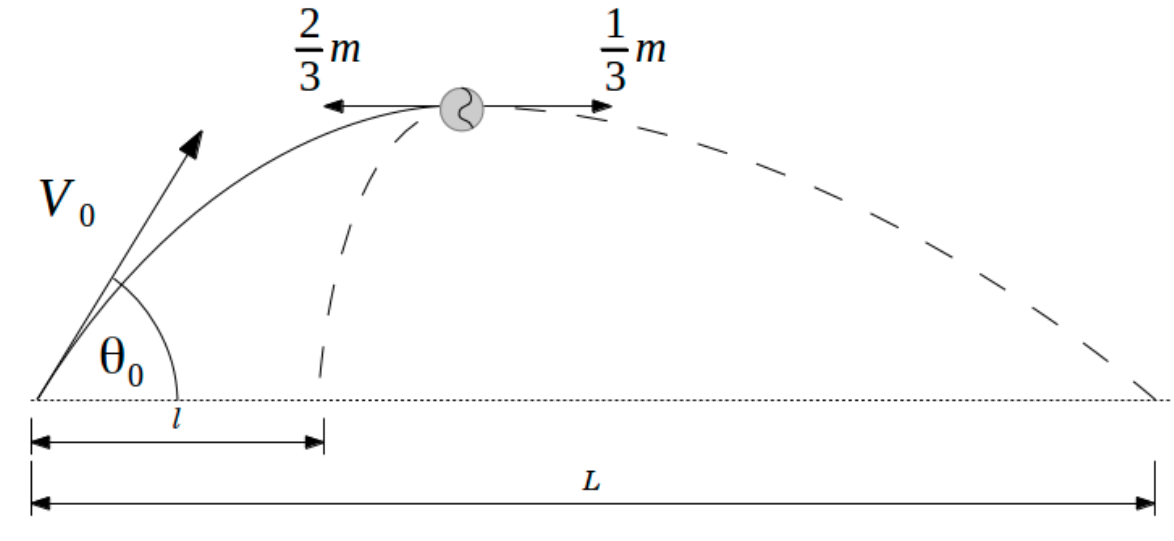
\includegraphics[width=0.4\linewidth]{2021-2/img/aux11/proyectil.PNG}
\end{figure}

\item Una argolla de masa $m_1$ que se mueve con rapidez $v_0$ (desconocida), se adhiere a una argolla de masa $m_2$ unida a un bloque de masa $M$ mediante un resorte de constante elástica $k$ y largo natural $L_0$. Inicialmente, la argolla $m_2$ está en reposo y el resorte se encuentra en posición vertical y en su largo natural. El bloque descansa sobre una superficie horizontal rugosa. A consecuencia de la colisión, las argollas continúan moviéndose juntas hasta detenerse cuando el resorte forma un ángulo $\theta$ con la vertical.
    
\begin{multicols}{2}
    \begin{enumerate}
        \item Determine la velocidad $v_0$ de la argolla $m_1$
        \item Determine el coeficiente de roce estático $\mu$ para que el bloque $M$ no resbale durante el movimiento de las argollas 
    \end{enumerate}
    \columnbreak
    \begin{figure}[H]
        \centering
        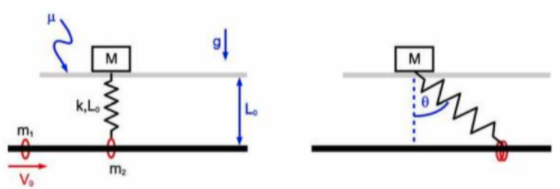
\includegraphics[width=0.8\linewidth]{2021-2/img/aux11/aa.PNG}
    \end{figure}
\end{multicols}
% Para imágenes vectoriales -> el texto tiene que estar en LaTeX
% \begin{figure}[htbp]
%   \centering
%   \svgpath{../Imagenes/ejercicios}  -> .. irse pa'trás 
%   \includesvg{ej5.svg}
% \end{figure}

\end{enumerate}
\end{document}